
	\subsection{Thesis Context}

		\begin{frame}
			\frametitle{Multimedia Information Retrieval}
			\only<1>{
				\centering
				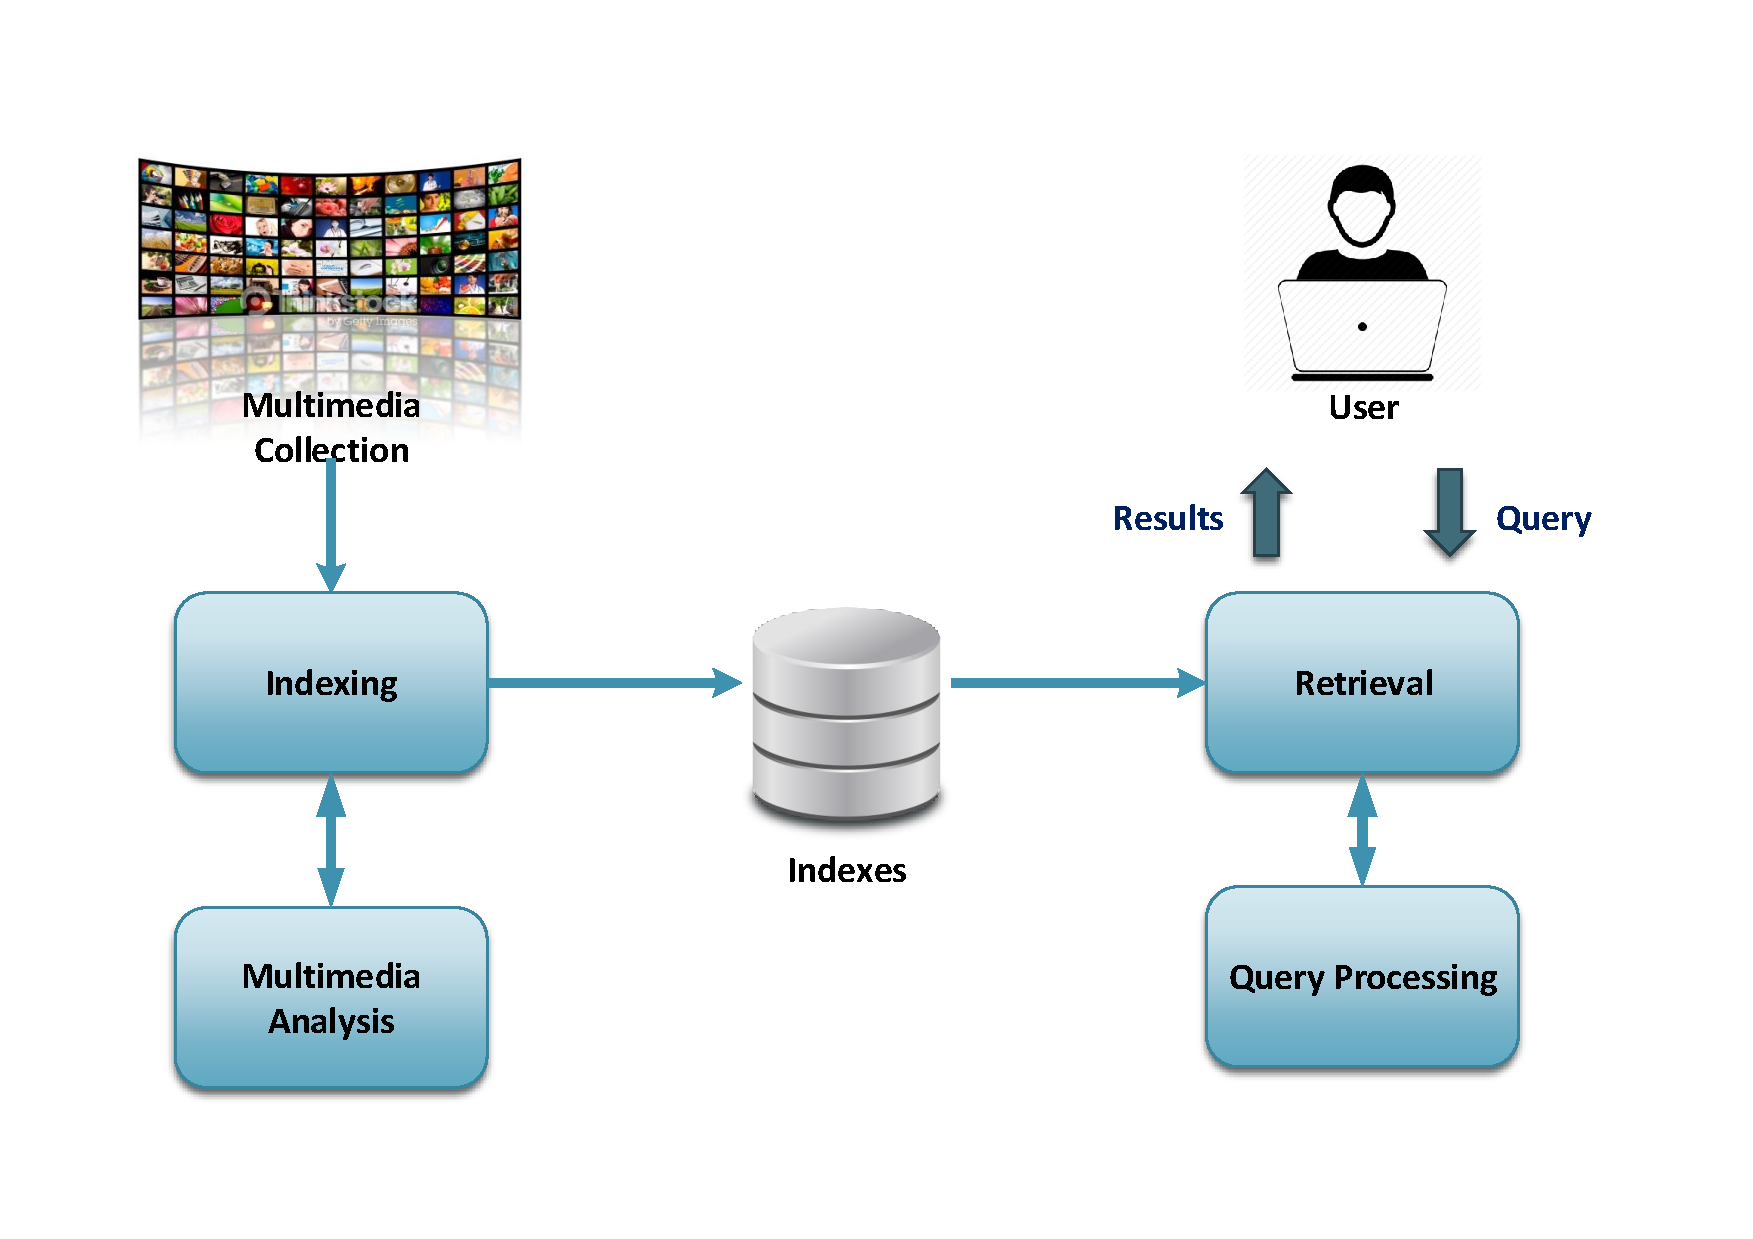
\includegraphics[scale=0.35]{graphics/p1_introduction_mir_1}	
			}

			\only<2>{
				\centering
		 		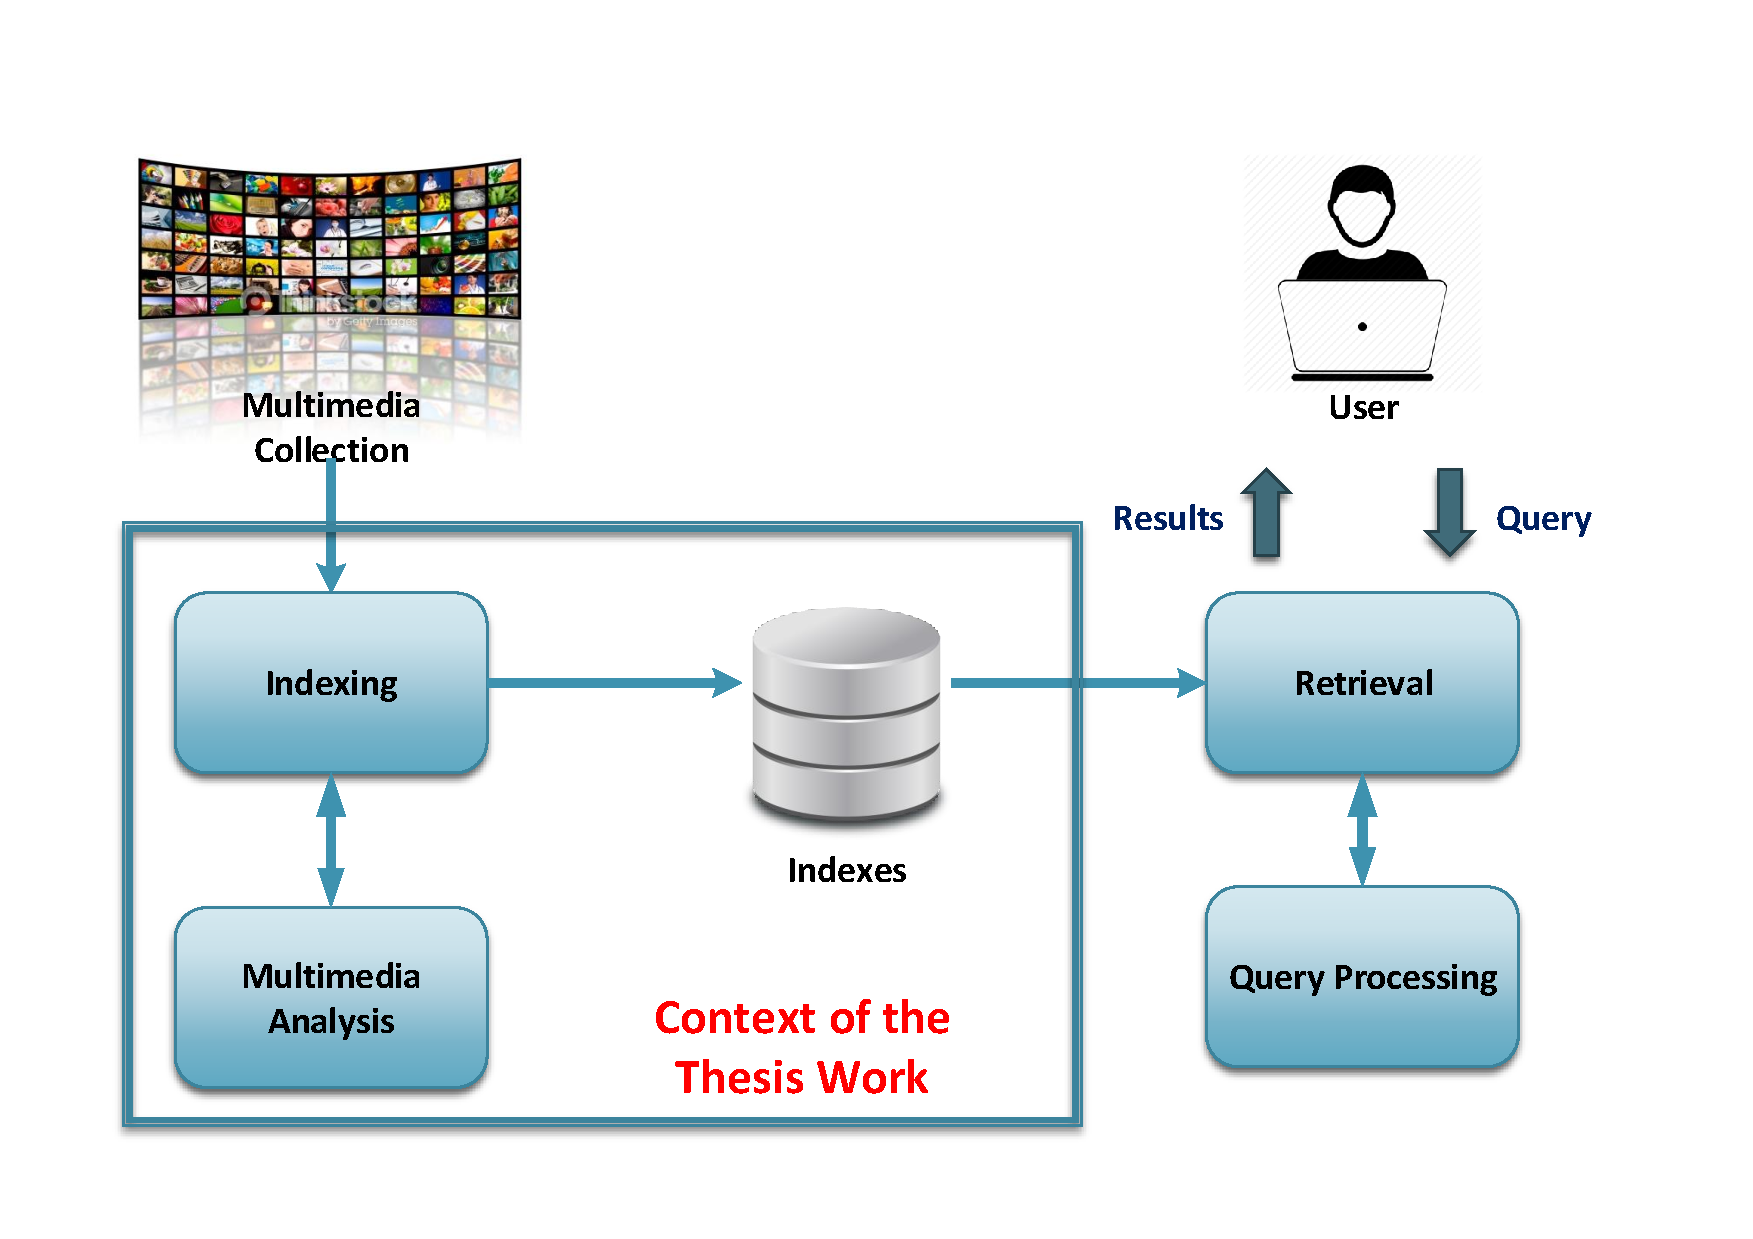
\includegraphics[scale=0.35]{graphics/p1_introduction_mir_2}
			}
		\end{frame}

		\begin{frame}
			\begin{center}
				\frametitle{Content-based Multimedia Indexing}
				{\only<1>{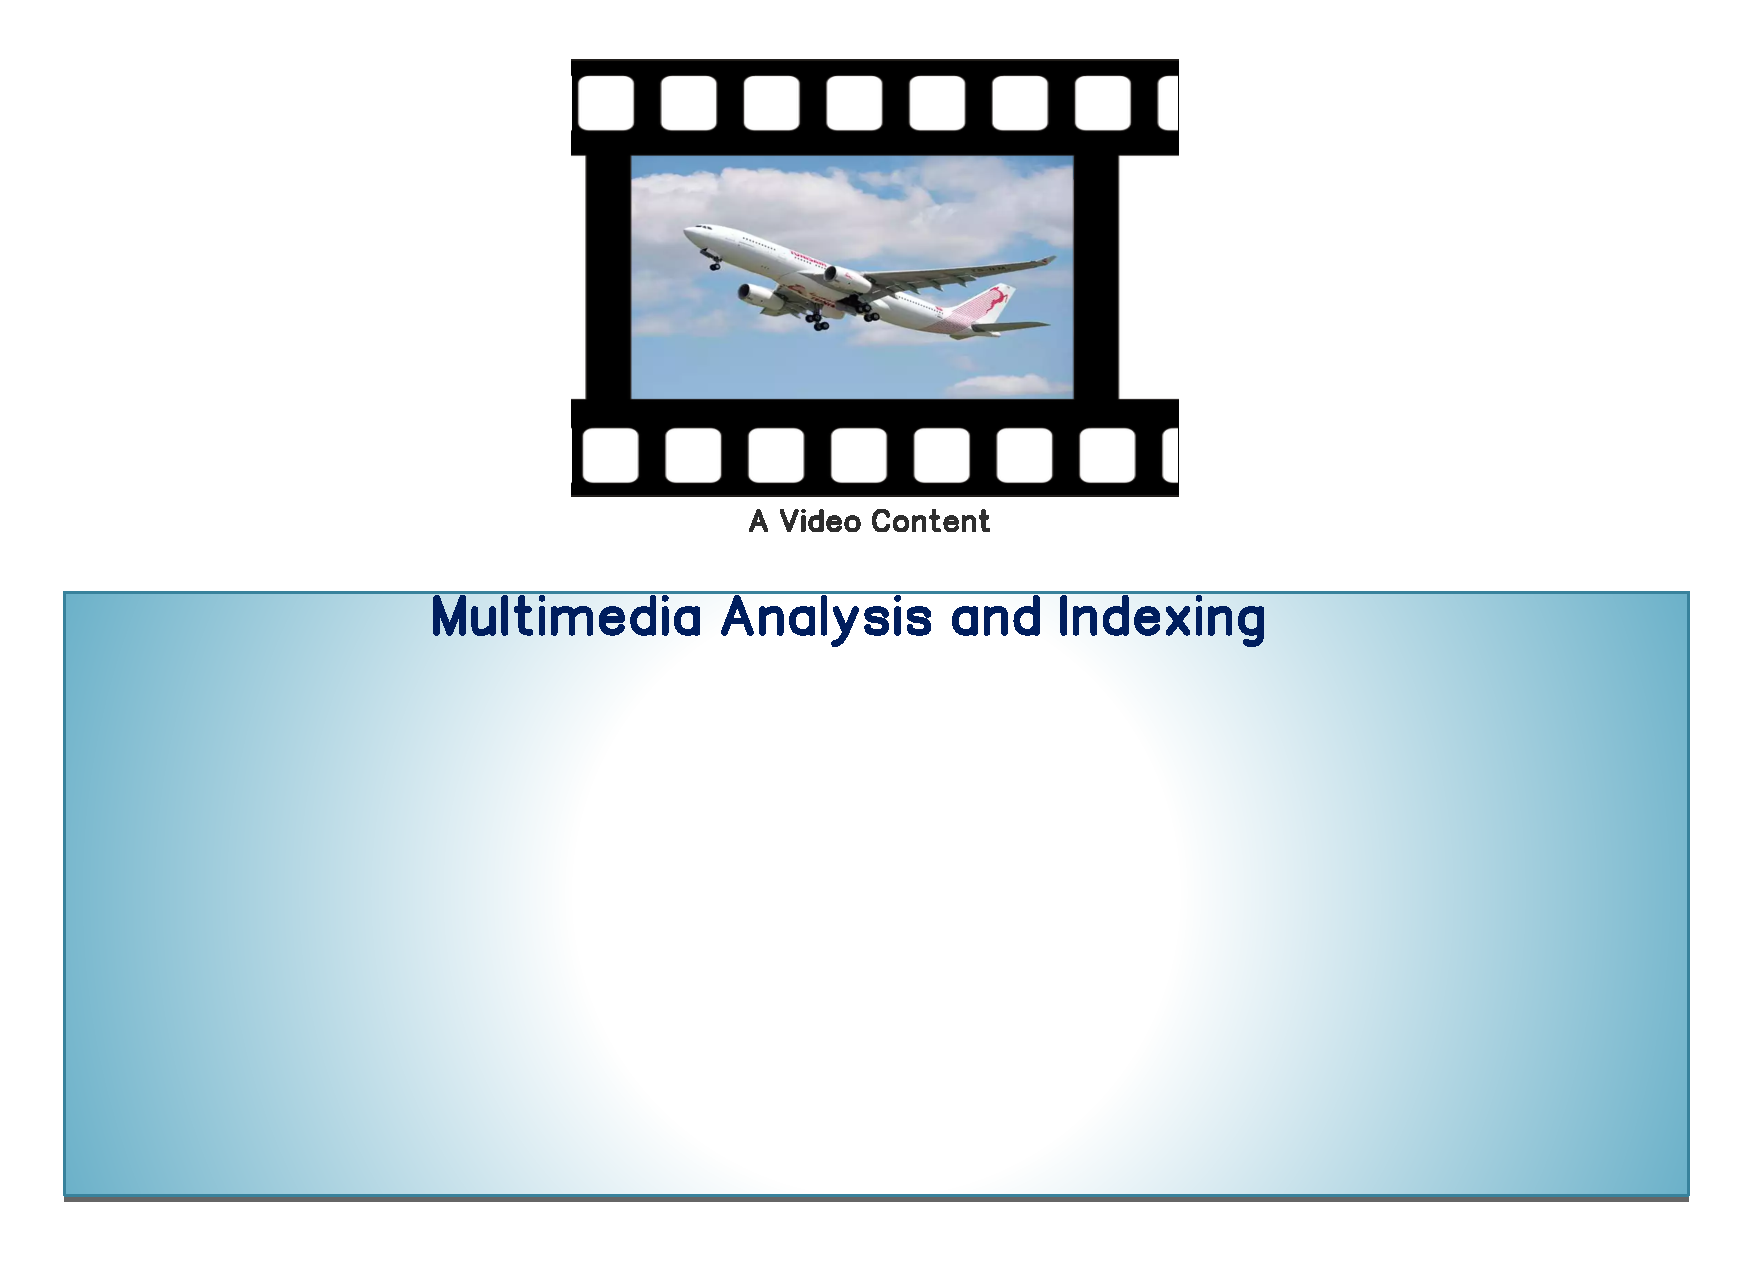
\includegraphics[scale=0.7]{graphics/cbmi1}}}
				{\only<2>{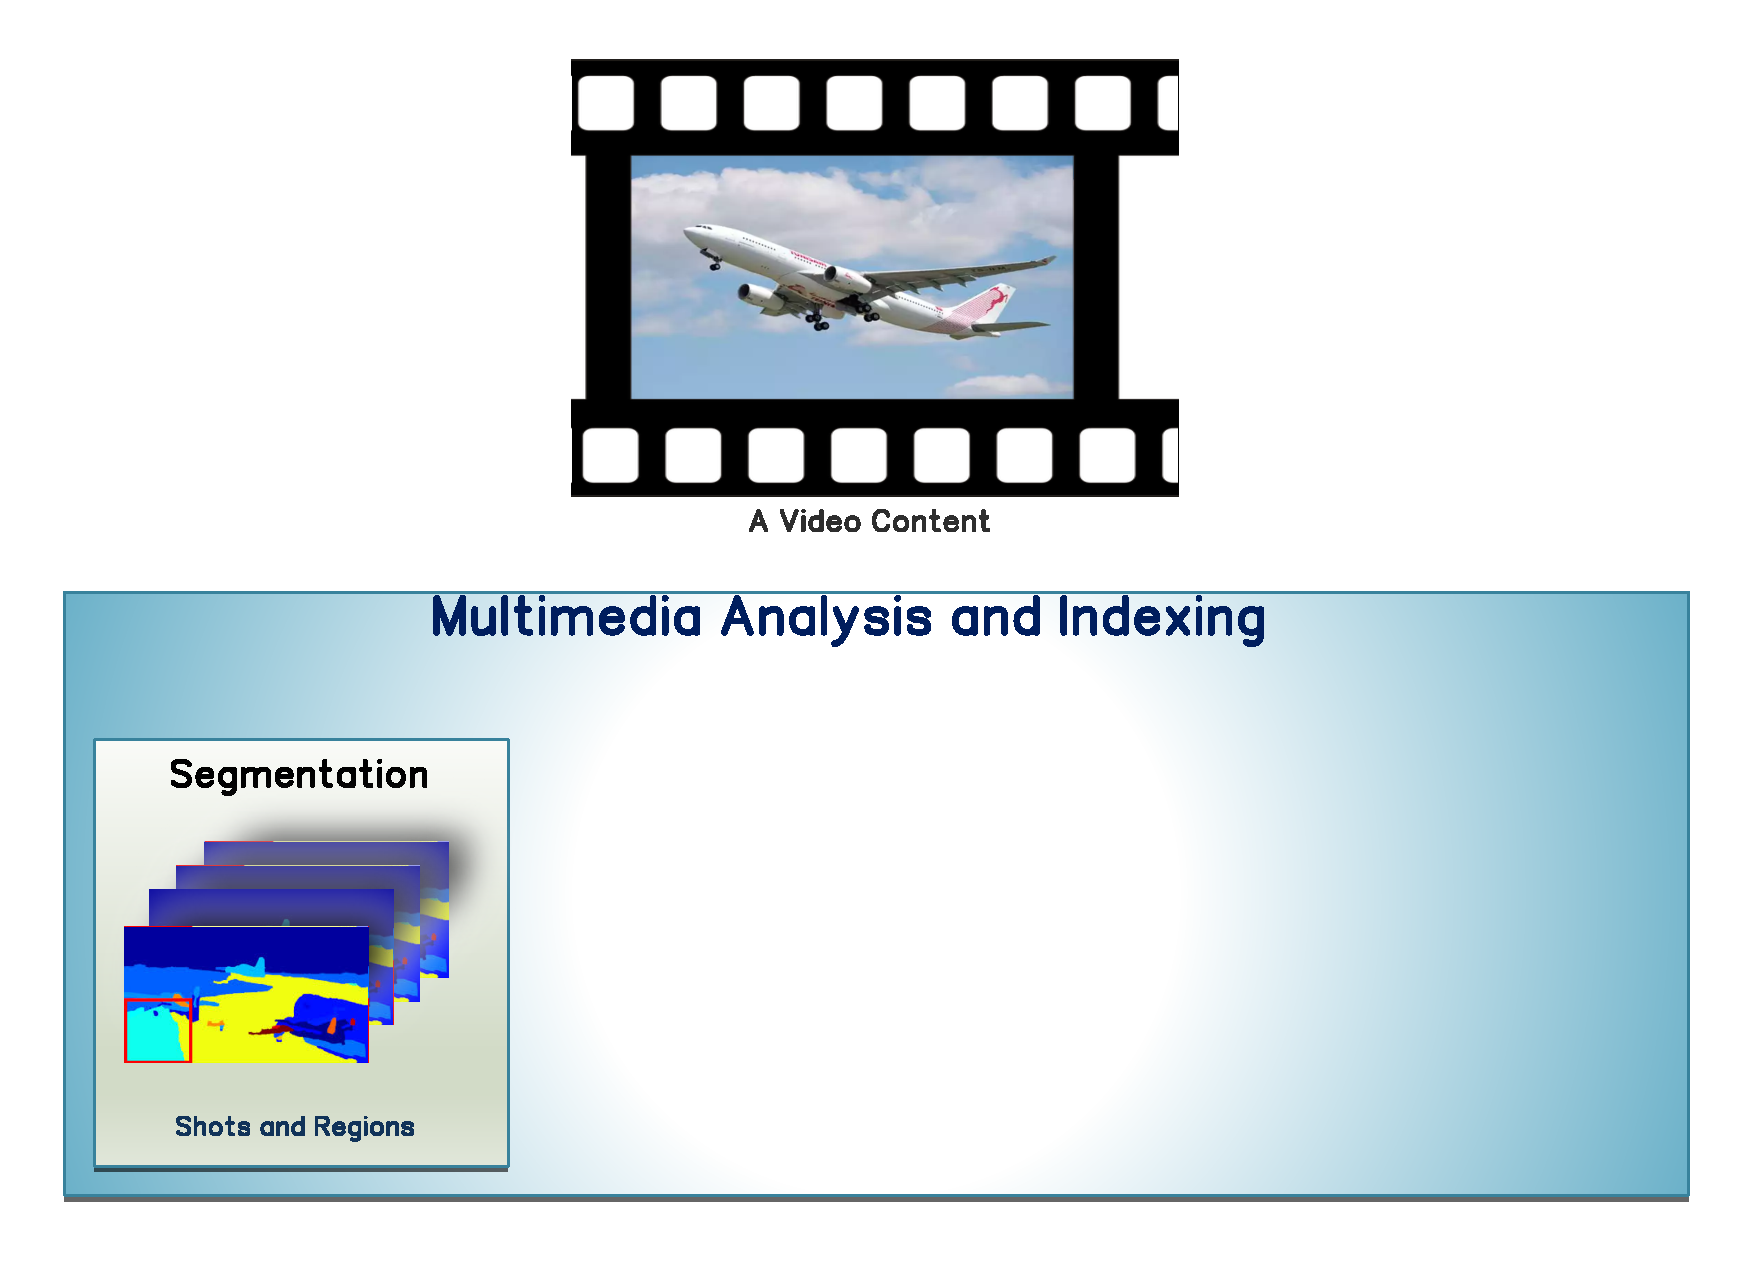
\includegraphics[scale=0.7]{graphics/cbmi2}}}
				{\only<3>{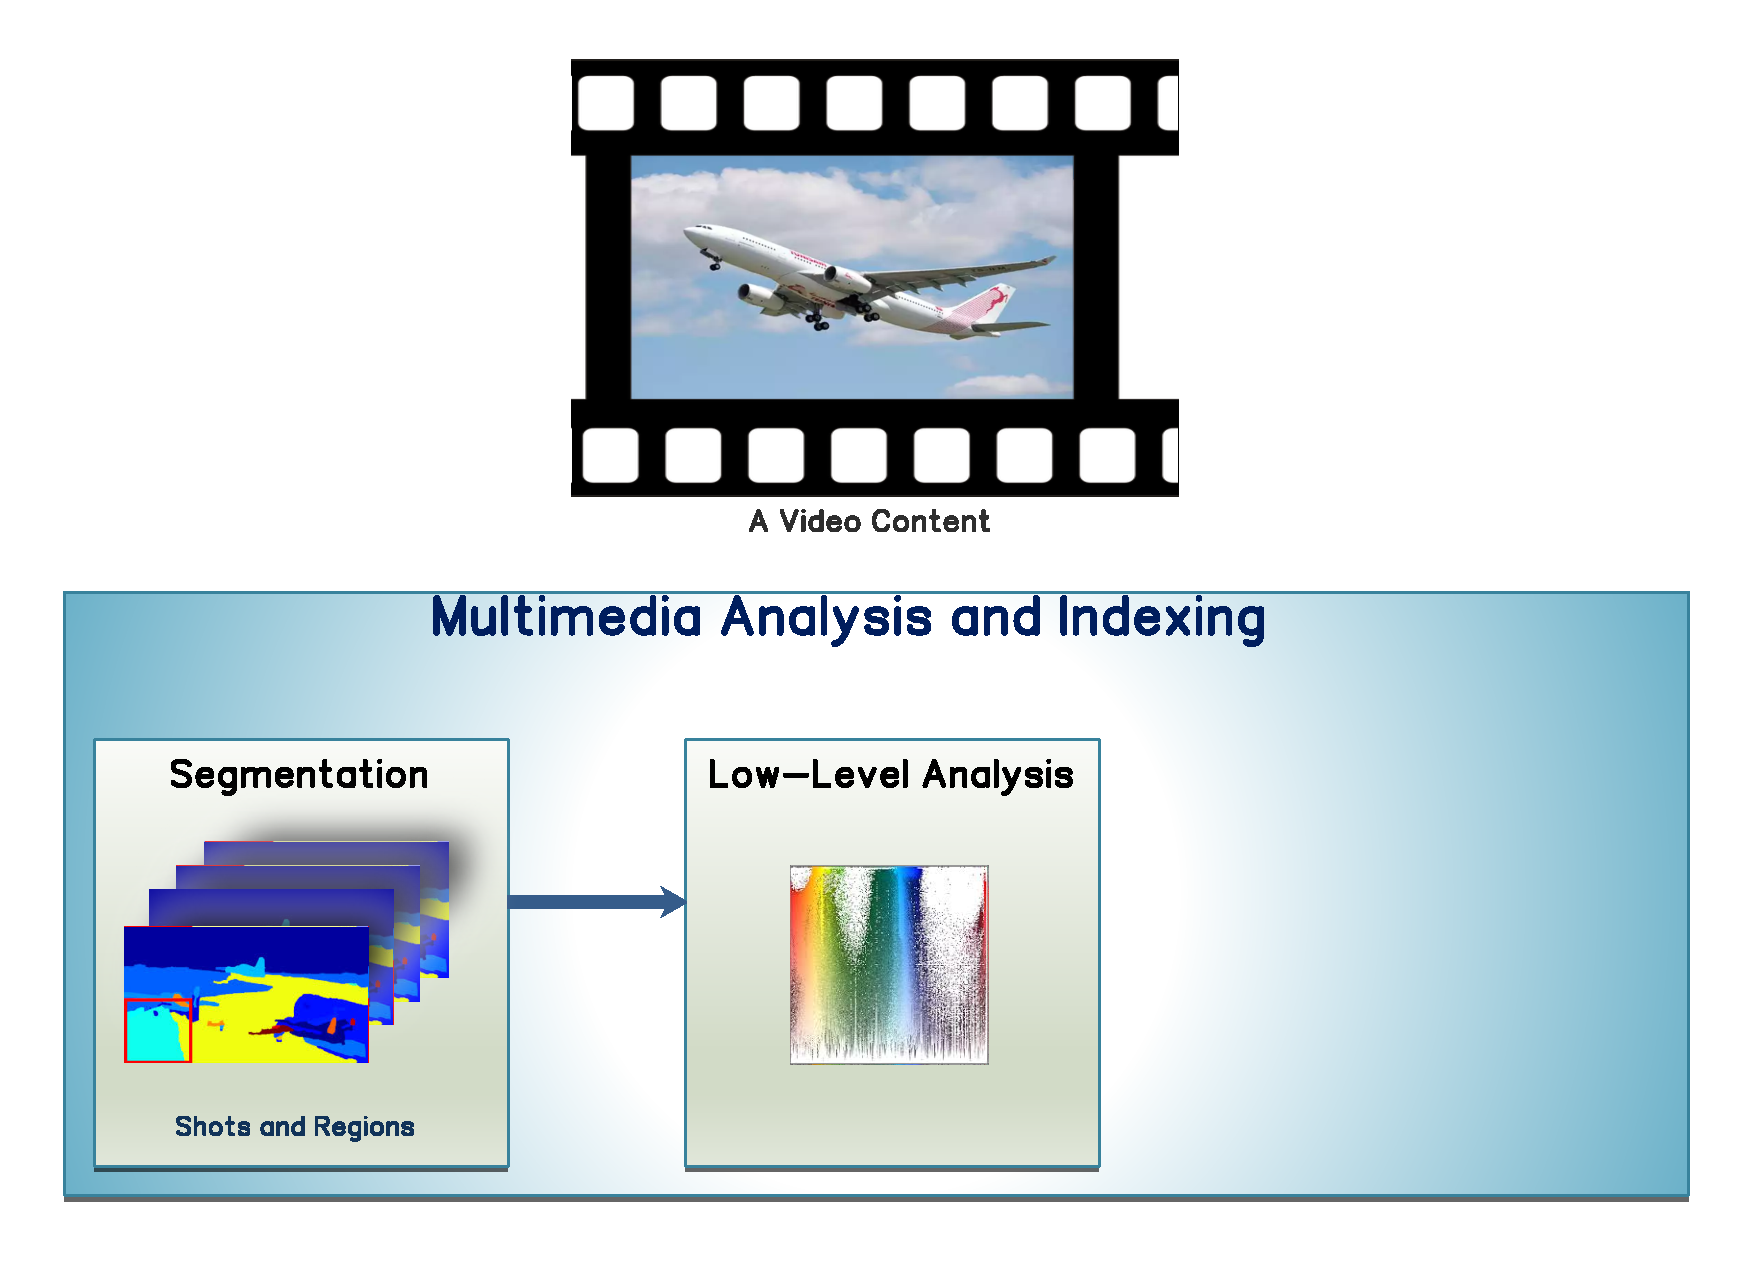
\includegraphics[scale=0.7]{graphics/cbmi3}}}
				{\only<4>{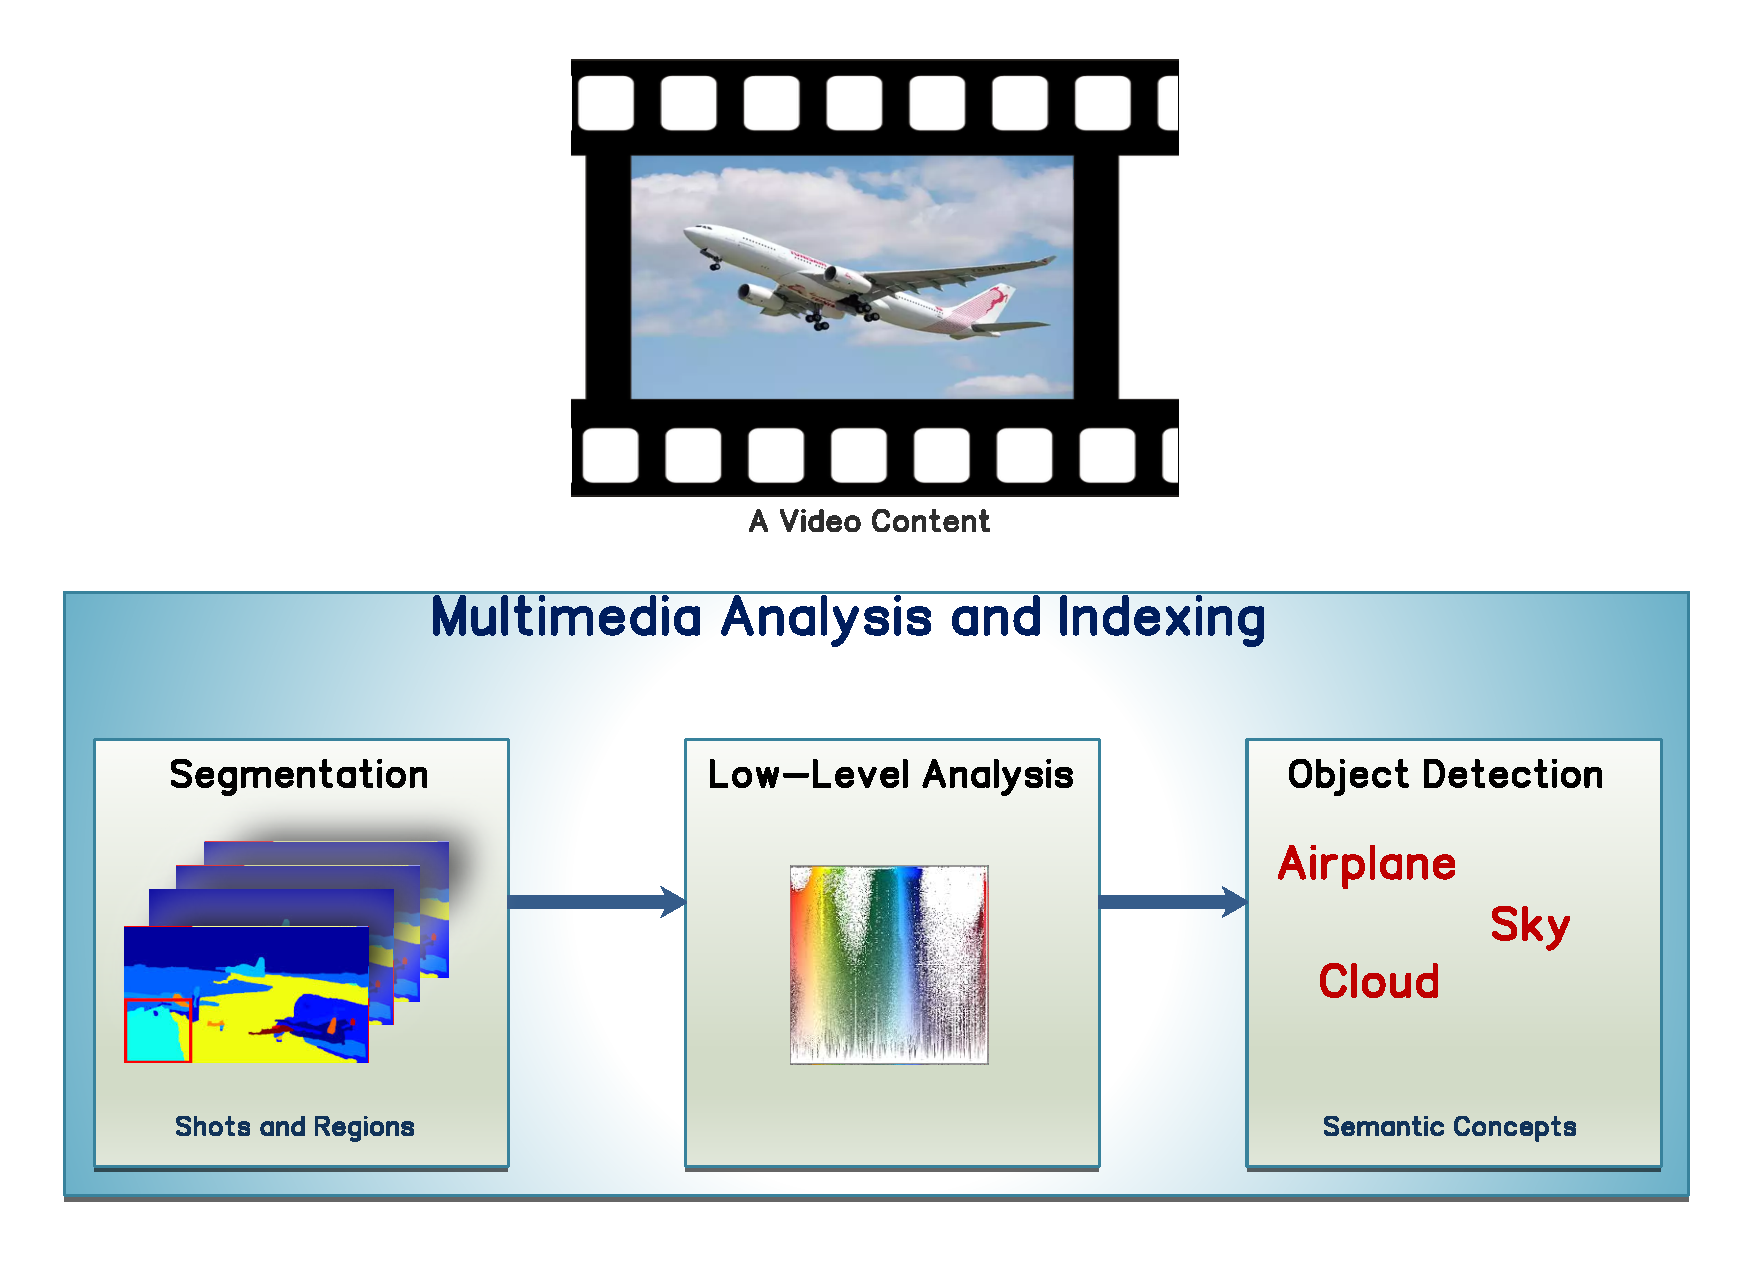
\includegraphics[scale=0.7]{graphics/cbmi4}}}
			\end{center}
		\end{frame}
		%\begin{frame}
		%	\frametitle{Content-based Multimedia Indexing}
		%	\animategraphics[autoplay,loop,width=0.5\textwidth]{4}{graphics/animated/airplane/*-}{0}{20} 
%
		%\end{frame}
	\subsection{Problems and Motivations}
		\begin{frame}
			\frametitle{Issue 1: Semantic Gap}
			\begin{block}{The semantic Gap}
				\begin{itemize}
					\item Concept detectors handle explicite information,
					\item The context of the content could give more information on present semantic object.
				\end{itemize}
			\end{block}
     			\begin{exampleblock}{}
			\only<1>{
				\centering
	 			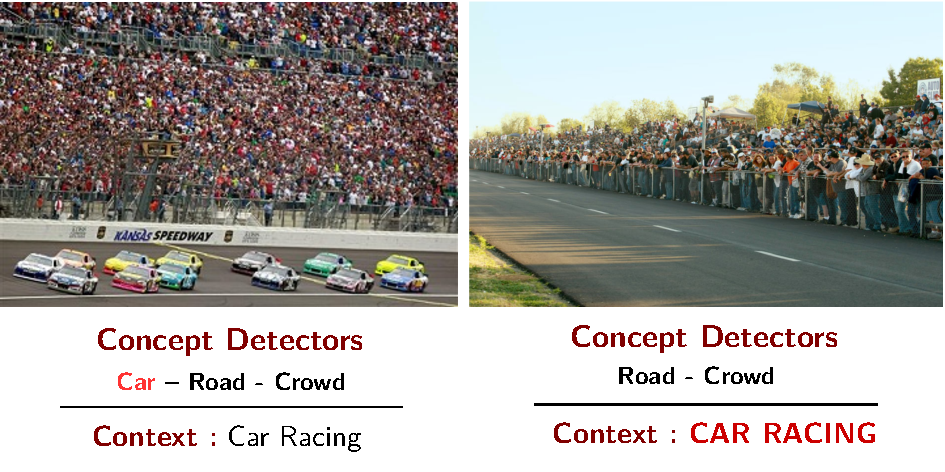
\includegraphics[scale=0.45]{graphics/issue1}
			}
			\only<2>{
				\centering
	 			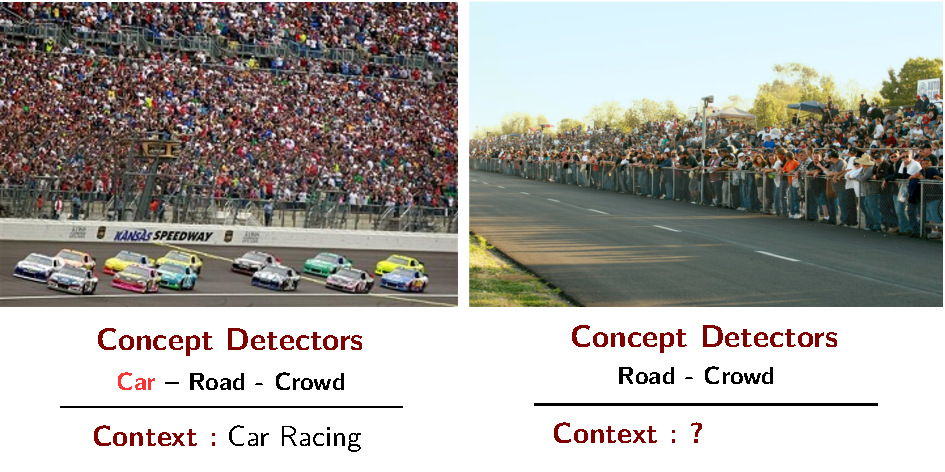
\includegraphics[scale=0.45]{graphics/issue1_1}
			}
			%\only<3>{
			%	\centering
	 		%	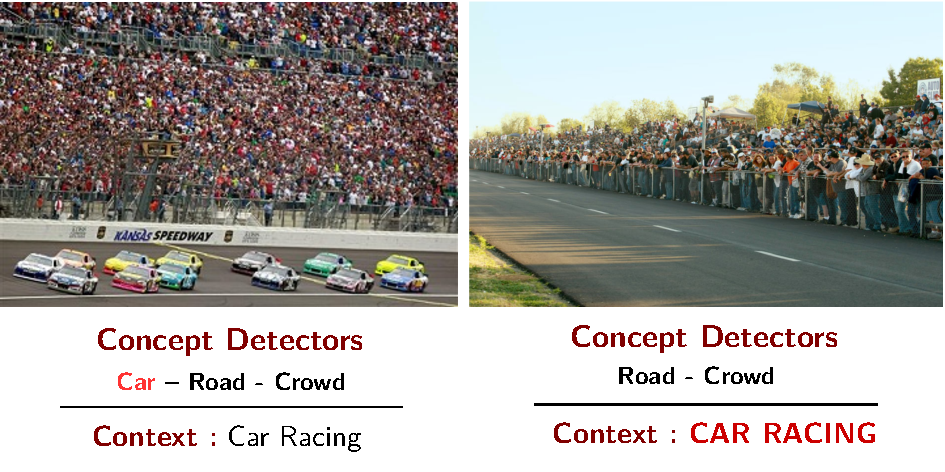
\includegraphics[scale=0.45]{graphics/issue1_2}
			%}
			\end{exampleblock}
			\end{frame}

		\begin{frame}
			\frametitle{Issue 2: Uncertianty}
			\begin{block}{The semantic Gap}
				\begin{multicols}{2}
					\begin{itemize}
						\item Multimedia content are often uncertain
						\item The door is \alert{too small} or the man is \alert{very tall} ?
						\pause
						\item In multimedia indexing, the uncertainty relies on handling
						 an incomplete interpretation 
						{\only<1>{\includegraphics[scale=0.6]{graphics/uncertain}}}
						{\only<2>{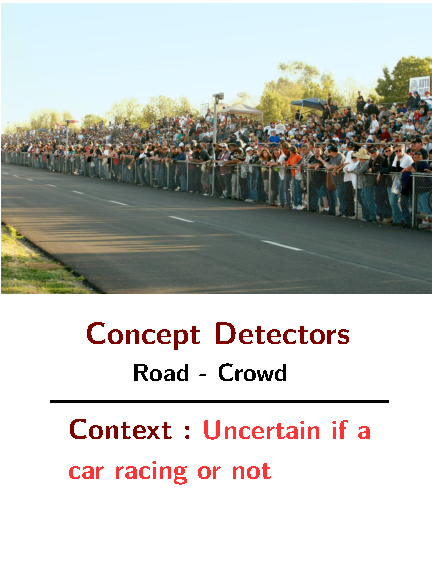
\includegraphics[scale=0.6]{graphics/uncertain_2}}}
					\end{itemize}
				\end{multicols}
			\end{block}
		\end{frame}

		\begin{frame}
			\frametitle{Issue 3: Scalability}
			\begin{itemize}
				\item Online multimedia data, images and video are overflowing our everyday life
				\item \alert{Flickr} stores over 5 billion of images and records an uploading 
					rate of over 3000 images per minute (2010)
				\item \alert{YouTube} records a rate of 300 hours of uploaded videos per minute
			\end{itemize}

			
			\pause
			\begin{alertblock}{}
				A crucial need for efficient tools to access to such amount of multimedia content
			\end{alertblock}
		\end{frame}

		\begin{frame}
			\frametitle{Opportunities}
			\begin{itemize}
				\item \alert{Fuzzy Knowledge} could improve machine based semantic analysis capabilities
				\item \alert{Semantic web}: many works are focused on managing knowledge for semantic content analysis
				\item \alert{Ontology} is a powerful tool for managing Knowledge and for inferring new ones
				\item \alert{Annotated video datasets} and Public \alert{multimedia web-services}
					are valuable data sources for extracting valuable knowledge
				\item \alert{Concepts interdependency} could be explored to reduce the indexing computing cost
			\end{itemize}	
		\end{frame}

		\begin{frame}
			\frametitle{Motivation}
			\begin{itemize}
				\item Reducing the semantic gap through providing an \alert{effective knowledge based 
					framework for enhancing a semantic interpretation}
				\item Reducing the uncertainty through the use of \alert{fuzzy reasoning framework}
					with the aim of assessing the consistency of the indexing process
				\item Ensuring the \alert{scalability} aspect through handling hierarchical 
					indexing process which scales well with large-scale multimedia content.
			\end{itemize}	
		\end{frame}
